\cleardoublepage\chapter{Related Work}\label{sec:related_work}\minitoc\vspace{.5cm}\index{SotA}

The concept of multipath is well-established, and in this section, we will explore notable existing multipath protocols, their characteristics, and highlight the unique aspects of our concept. 
Additionally, we will discuss future use cases for our \ac{MTX} and examine current solutions and technologies being utilized. 
Finally, we will take a closer look at the design of the 5G system, with a specific focus on the Data Plane, to explain our plan for showcasing the multipath tunnel using the \ac{gptu} protocol.

\section{Tunneling}\index{Tunneling}
\todo{these following are my words, but do I need cite here?}
The concept of a tunnel draws inspiration from its real-world counterpart, which refers to a confined pathway constructed to direct transportation between two points, separate from the surrounding terrain. 
In the physical sense, tunnels are often excavated deep beneath the earth's surface to bypass obstacles like mountains, rivers, or ocean channels.
In the realm of networking, a tunnel can be perceived as a direct network pathway that enables access to another network from the network to which it is currently connected. 
From an infrastructure standpoint, a tunnel serves as an abstraction layer that abstracts the actual traffic routing from the application and isolates the tunnel's traffic from public network traffic. 
This is typically achieved by encapsulating the application's data packets within the tunnel's packets, and then extracting the original data at the other end of the tunnel.
Many tunnel protocols exist for different purposes: IPv4/IPv6 tunnels to enable compatibility between exclusive networks \cite{rfc4380_Teredo_ipv6_tunnel_udp}, Secure Shell (SSH) - tunnel for remote access and data transfer \cite{rfc4251_ssh_protocol}, and \ac{VPN} tunneling - used for access other network from another network. 
\ac{VPN}s are frequently utilized to remotely access a private network, such as connecting to university's network from home. 
It also functions to conceal the origin of network traffic by making it appear as if it originates from the VPN server, which is useful for bypassing firewalls or restrictions applied by local network providers.
The traffic can also be encrypted to add an extra layer of protection while accessing networks over untrusted connections, like public WLAN provided by coffee shops.
There are several widely recognized VPN protocols, including WireGuard, OpenVPN, IPsec, Cisco AnyConnect VPN, L2TP/IPsec, SSTP (Secure Socket Tunneling Protocol), ... each embodies its unique philosophy, background, and intended field of application.


\section{Multipath Connection}\index{Multipath Connection}\label{sec:related_work:mp_connection}
Our primary emphasis is on establishing a connection between two points, irrespective of the number of physical transportation links.
% We will explore various protocols that implement the concept and make comparisons with our approach.
There are 2 approaches to utilize multiple links: managing multiple underlying connections created by existing protocols (\ac{MPTCP} with TCP), and creating a new multipath protocol (\ac{SCTP}).
Drawing inspiration from these protocols, our design of \ac{MTX} adopts a hybrid approach: a tunnel that transfers data over multiple UDP connections instead of maintaining TCP sessions. 
The tunnel data path comprises two primary logical stages: the data stage and the transport stage. 
The data stage handles session management, congestion control overhead, and other administrative tasks, enabling the transport stage to be constructed with wrappers over UDP sockets.
Unlike serving solely the caller, the multipath tunnel is designed to offer connection and flow management for multiple applications, enabling centralized resource management and scheduling.

\subsection{Multipath TCP}\label{sec:related_work:mp_connection:MPTCP}
% MultiPath TCP (MPTCP) is an effort towards enabling the simultaneous use of several IP-addresses/interfaces by a modification of TCP that presents a regular TCP interface to applications, while in fact spreading data across several subflows. Benefits of this include better resource utilization, better throughput and smoother reaction to failures. 

\ac{MPTCP} is is a major extension to TCP to decoupling TCP from the transport layer by utilizing multiple sub flows, which are underlying TCP connections \cite{Bonaventure_mptcp_decoupling}.
The protocol is showcased in both mobile and data center environments, serving distinct objectives. 
In addition to enhancing data center performance by employing \ac{MPTCP}'s distributed load-balancing across multiple paths, the protocol also provides redundancy and effective congestion management capabilities \cite{raiciu_improving_nodate}.
In the context of mobile hand-over capability, \ac{MPTCP} enhances the ability to maintain TCP sessions while the user equipment moves continuously. 
For instance, a smartphone can continue utilizing both LTE and Wi-Fi connections for a TCP session and predict the optimal route for transmitting most of the traffic. 
By monitoring the radio signal strength, it becomes possible to anticipate potential disruptions in the Wi-Fi connection or when a user enters a building and encounters a loss of cellular signal. 
The author argues that although maintaining two radios simultaneously consumes more power, it can potentially reduce the time required to establish new connections and transmit data \cite{paasch_multipath_2014}.

\begin{figure}[H]
	\centering
	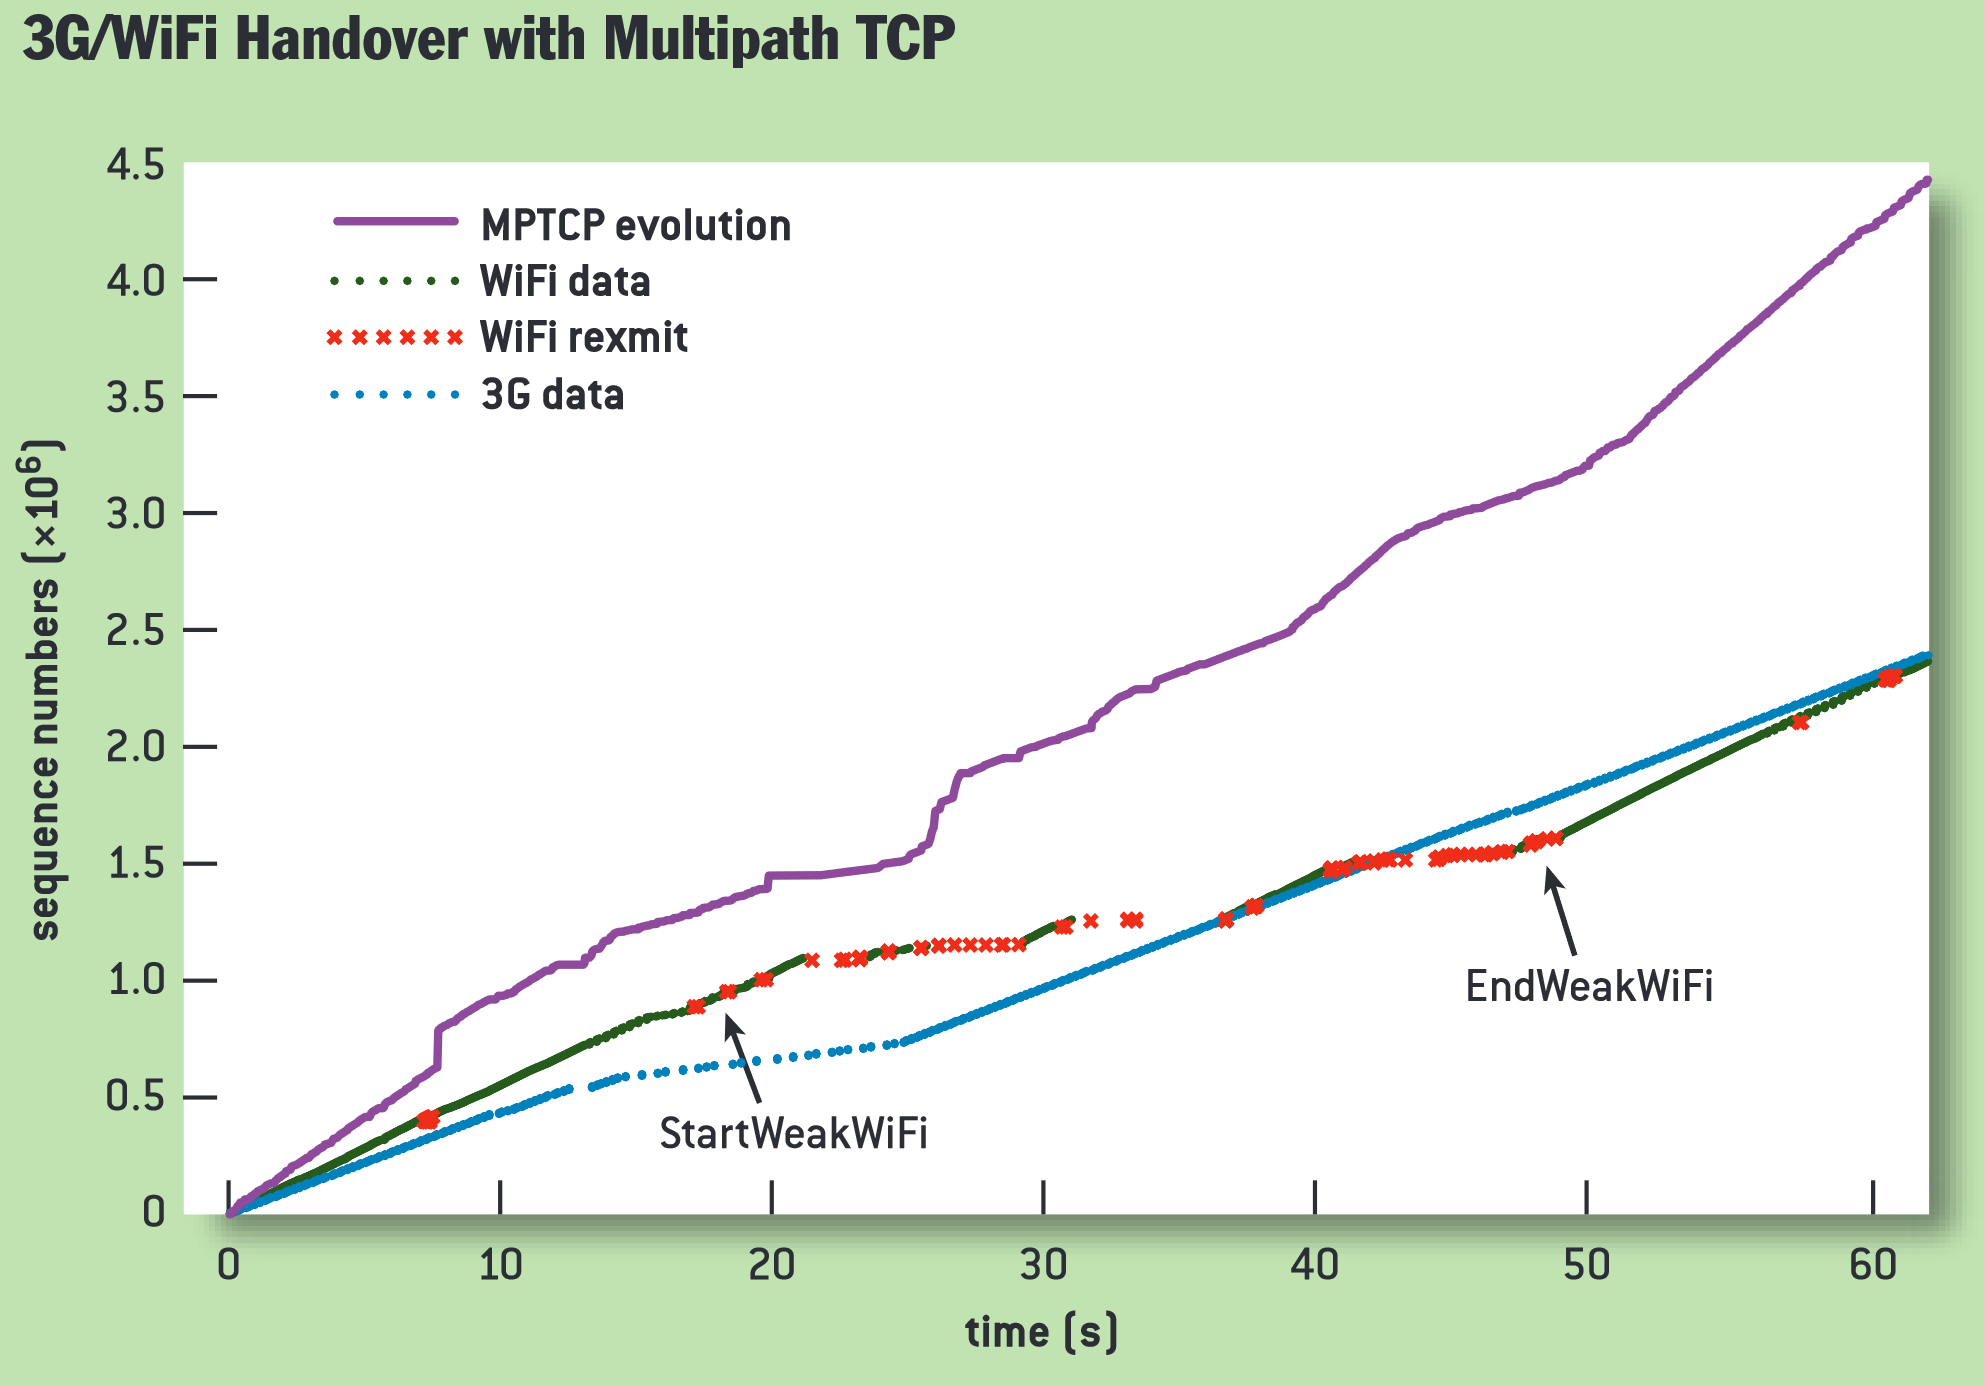
\includegraphics[width=1.0\textwidth]{resources/images/3G_WiFi_Handover_with_Multipath_TCP.PNG}
	\caption{3G/WiFi Handover with Multipath TCP \cite{paasch_multipath_2014}. The MPTCP connection (in violet) persists despite of WiFi and 3G's unreliable connections. A weak WiFi signal can be indicative of the device moving beyond the coverage range of the router. The command \textit{REXMIT} changes the time-out value for each packet which is used for retransmitting packet. This indicates the TCP connection was trying to retransmit over the weakening WiFi connection.}
    \label{fig:related_work:3G_WiFi_Handover_with_Multipath_TCP}
\end{figure}

\subsection{Stream Control Transmission Protocol}\label{sec:related_work:mp_connection:SCTP}
\ac{SCTP} introduces multiple addresses to the transport layer, which serves as failover and simultaneous underlying connection.
Unlike \ac{MPTCP}, existing internet's infrastructure such as firewalls, routers were not designed to handle \ac{SCTP}'s packets and thus severely limits usage of the protocol \cite{paasch_multipath_2014}. 
Notably, \ac{SCTP} is used in 5G core design for transmitting messages in Control plane.

\begin{figure}[H]
	\centering
	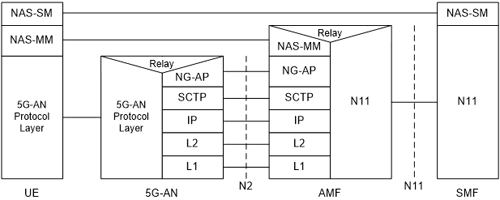
\includegraphics[width=0.8\textwidth]{resources/images/3gpp_5g_part_of_control_plane_protocol.png}
	\caption{3GPP: Control Plane protocol stack between the UE, the 5G-AN, the AMF and the SMF \cite{3gpp_5g_system_overview}}
    \label{fig:related_work:3gpp_5g_part_of_control_plane_protocol}
\end{figure}


\section{5G Deployment}\index{5G Deployment}
5G services and functions are designed to be deployed in containers and virtual machines, often on server-grade general purpose computers.
These components are categorized into two groups: the Control plane and the Data plane (\Cref{fig:related_work:Non_Roaming_5G_System_Architecture_in_reference_point_representation}).

\begin{figure}[H]
	\centering
	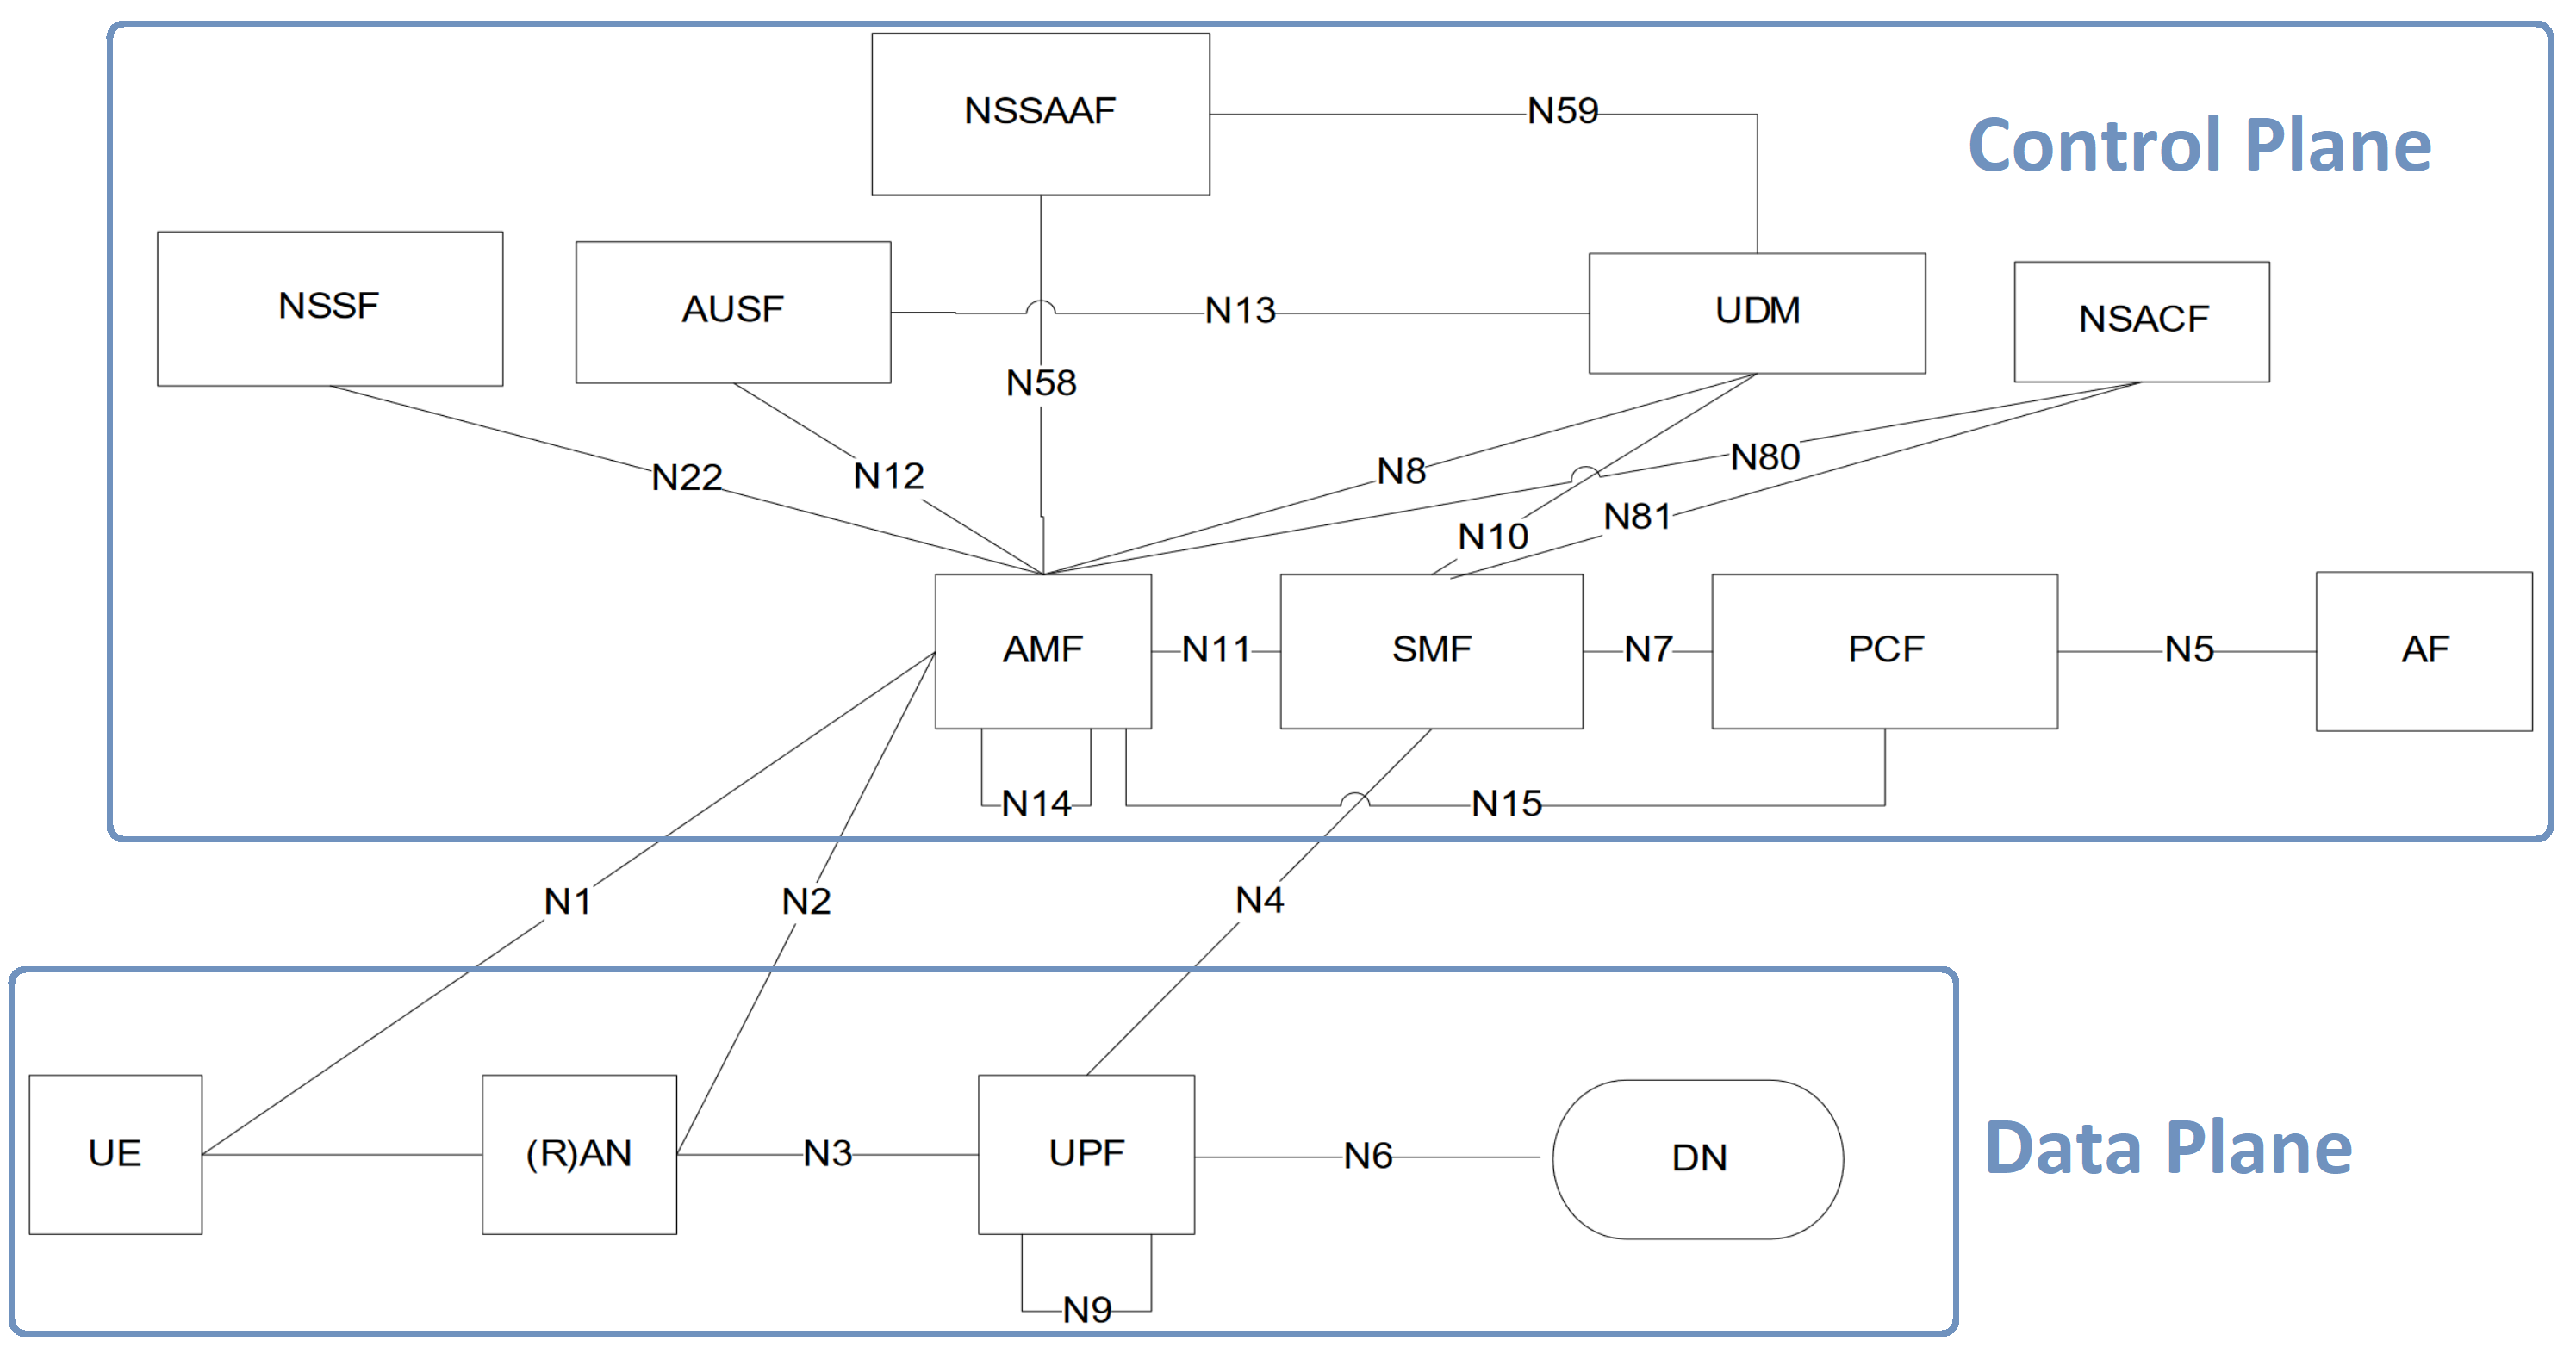
\includegraphics[width=1.0\textwidth]{resources/images/Non_Roaming_5G_System_Architecture_in_reference_point_representation.png}
	\caption{Data and Control Plane in 3GPP's Non-Roaming 5G System Architecture in reference point representation \cite{3gpp_5g_system_architect_spec_release_18}}
	\label{fig:related_work:Non_Roaming_5G_System_Architecture_in_reference_point_representation}
\end{figure}

As mentioned in \Cref{sec:related_work:mp_connection:SCTP}, the control plane uses \ac{SCTP} protocol with multipath support for its internal communication.
The Data plane relies on \ac{gptu} protocol with \ac{UDP} as the transport protocol to deliver high volume of data between \ac{UE} and \ac{DN} (see \Cref{fig:introduction:3gpp_5g_data_plane_protocol}), which require powerful processing power and high capable network link.
According to \ac{3GPP}, an non-exhausted list of \ac{UPF}'s responsibility is \textit{packet routing \& forwarding}, packet \textit{inspection}, \textit{buffering}, \textit{sending} and \textit{forwarding} \cite{3gpp_5g_system_architect_spec_release_18}.
In order to meet the \ac{SLA} and \ac{QoS} requirements, the \ac{UPF} needs to be deployed in various locations, such as the edge (edge and campus), regional sites, and central data centers \cite{zte_upf_full_whitepaper}. 
The size and form of each \ac{UPF} instance vary significantly depending on factors such as the number and size of downstream and upstream functions it manages and responds to, as depicted in \Cref{fig:related_work:Deployment_Requirements_of_Full_Scenario_UPF}.

\begin{figure}[H]
	\centering
	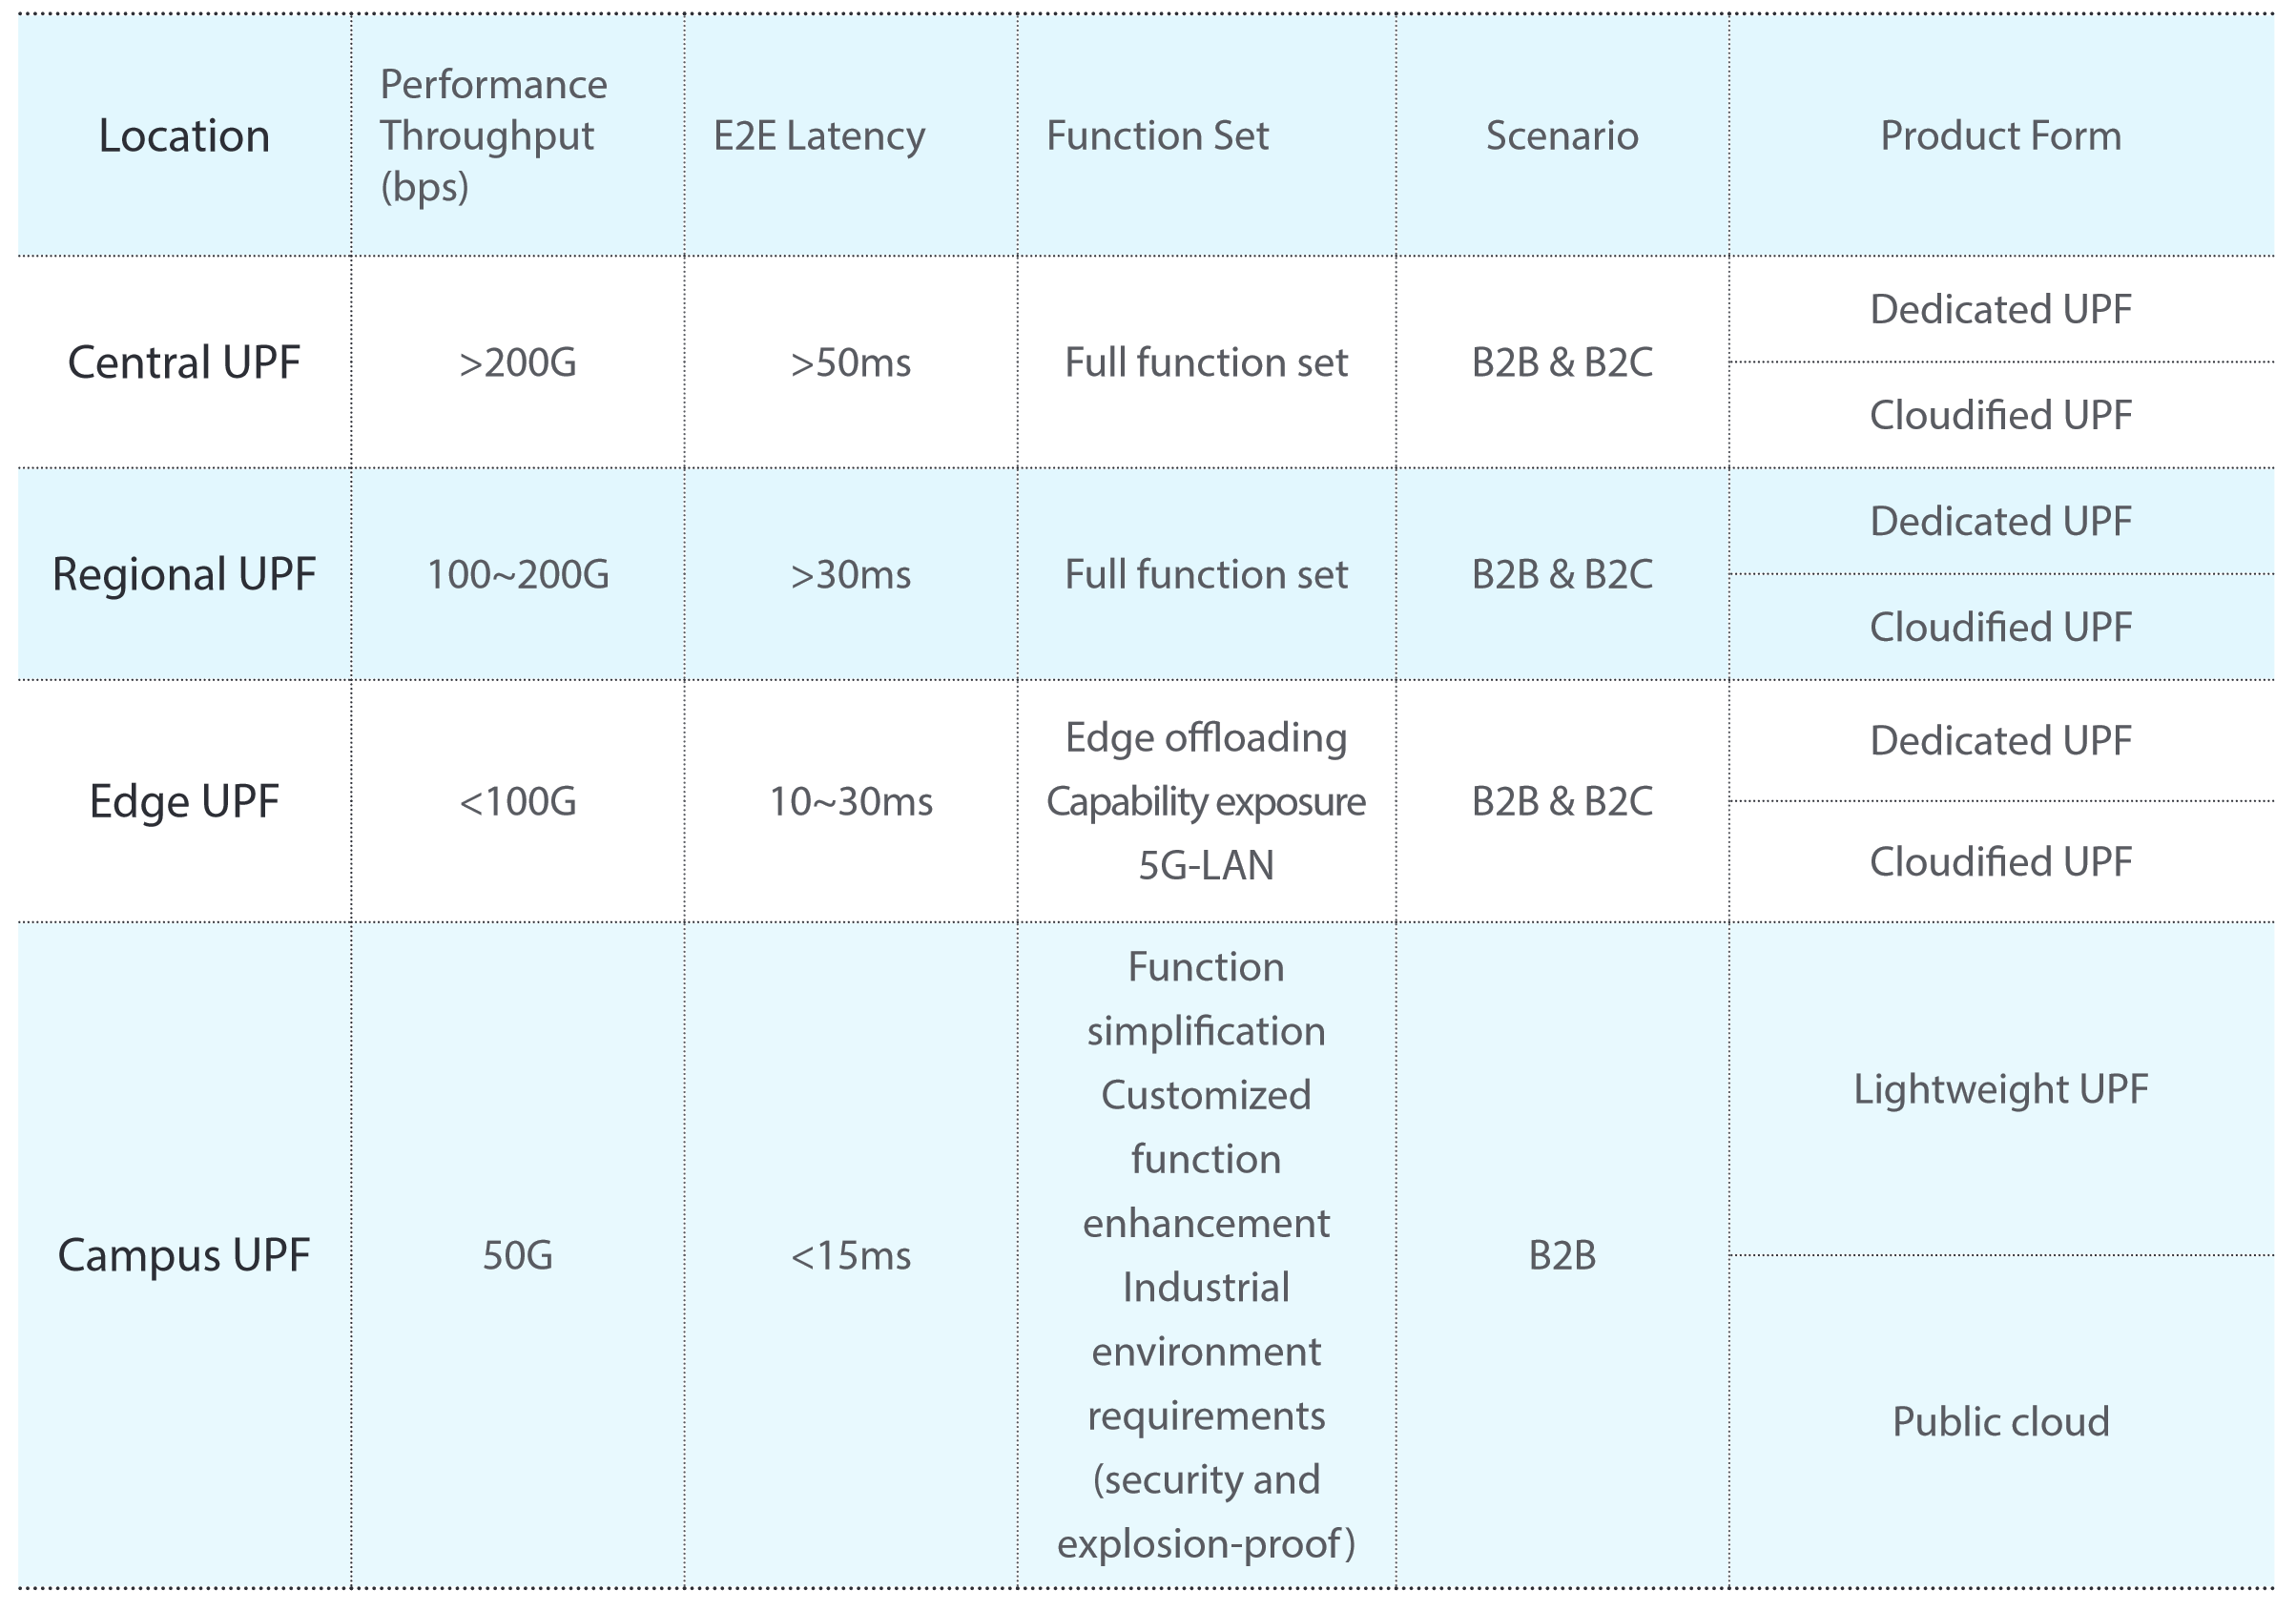
\includegraphics[width=1.0\textwidth]{resources/images/Deployment_Requirements_of_Full_Scenario_UPF.PNG}
	\caption{ZTE's White Paper: Deployment Requirements of Full-Scenario UPF \cite{zte_upf_full_whitepaper}}
    \label{fig:related_work:Deployment_Requirements_of_Full_Scenario_UPF}
\end{figure}

% Although no feature equivalent to multipath is built in the \ac{gptu} protocol, data plane's implementations come up with their own technology stack for high performance. 
While the \ac{gptu} protocol does not have a built-in feature equivalent to multipath, vendors have developed their own data plane technology stack to achieve high performance.
\ac{NEC} demonstrated its containerized \ac{UPF} solution's capability by handling 640Gbps bandwidth on 1 single 2x32 cores server \cite{nec_upf_whitepaper}.
\ac{dpdkpage} library was used to forward the enormous data flows to the containers (\Cref{fig:related_work:640_nec_upf_system}).
\ac{ZTE} offers hardware platforms and software stack that use a combination of \ac{dpdkpage}, \ac{sriov} and hardware acceleration technology to support a wide range of bandwidth capacity from 5Gbps to 200Gbps \cite{zte_upf_full_whitepaper}, and up to 462Gbps in a test scenario in cooperation with Intel \cite{zte_5g_core_upf_impl}.

Our \ac{MTX} library is positioned as an alternative to packet handling components based on \ac{dpdkpage} and \ac{sriov}. 
In the subsequent sections, we will introduce these two technologies and highlight the potential advantages offered by our solution.

\begin{figure}[H]
	\centering
	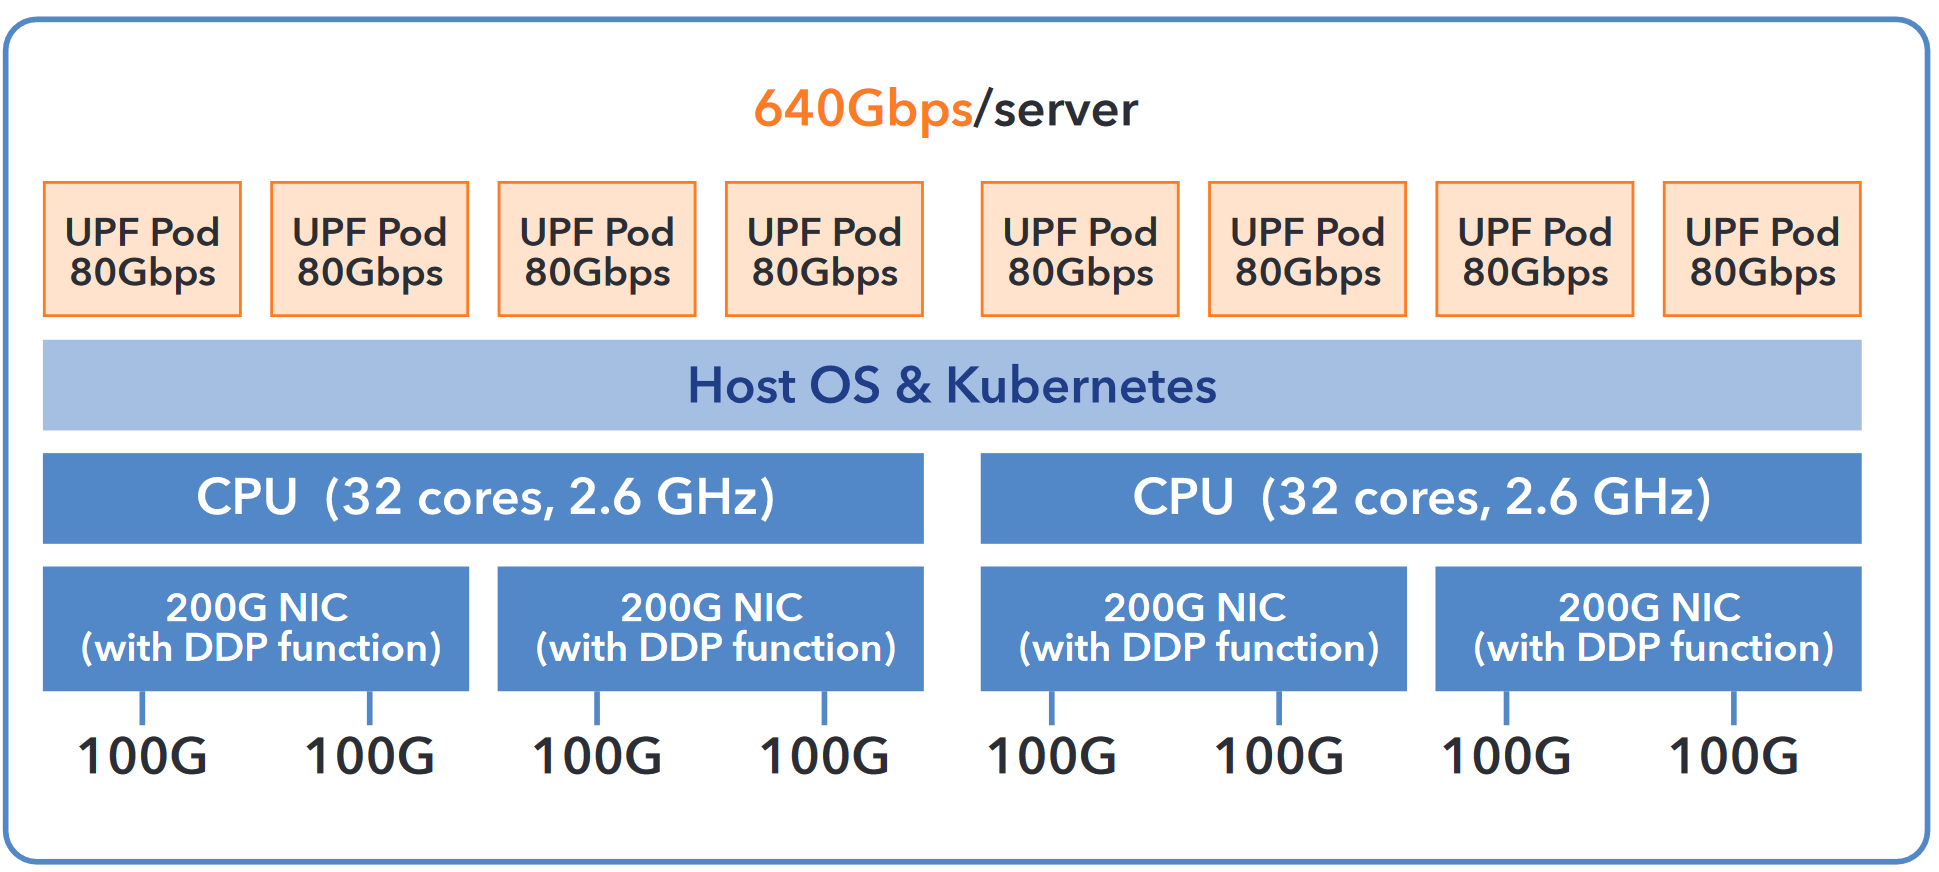
\includegraphics[width=1.0\textwidth]{resources/images/640_nec_upf_system.PNG}
	\caption{NEC's containerized UPF software (8 pods per server) on a platform configured with Linux and Kubernetes \cite{nec_upf_whitepaper}}
    \label{fig:related_work:640_nec_upf_system}
\end{figure}

\subsection{Data Plane Development Kit}
\ac{dpdkpage} is a library initially developed by Intel engineer Venky Venkatesan and currently maintained by the Linux Foundation. 
It provides a solution that contains a collection of libraries, poll drivers and configuration designed to accelerate packet processing workloads. 
By decoupling the NIC and CPU cores from the kernel, the library establishes a highly efficient and high-throughput data path, thus eliminates the overhead introduced by Linux kernel's network stack \cite{kourtis_enhancing_2015}. 
\ac{dpdkpage} has been widely utilized in various projects, including pfSense, Open vSwitch/OpenStack, Intel's DDP, OpenFlow, and 5G UPF implementations \cite{intel_ddp_ethernet_800}\cite{pongracz_removing_2013}\cite{zte_5g_core_upf_impl}\cite{nec_upf_whitepaper}. 
% Recently, the \ac{dpdkpage} team proposed a QoS plugin enhancement at the GTP-U packet stream level for UPF \cite{dpdk_upf_extension}.

From a technical standpoint, \ac{dpdkpage} is a kernel-bypassing method to process network packets that can deliver packets to application in user space with very low latency.
In addition, \ac{dpdkpage} offers a range of powerful features, including Crypto, DMA direct memory access, CUDA GPU utilization, and Machine Learning Device Driver \cite{dpdk_guide_page}. 
\ac{dpdkpage} is however, not a networking stack and has no Layer-3 forward, IPsec, firewall features \cite{old_dpdk_page} and forces developers to maintain their own code base for such purposes.
Therefore, using \ac{dpdkpage} in small open-source projects may necessitate more extensive maintenance and configuration compared to utilizing an in-kernel alternative like \ac{xdppage} socket, which will be utilized to construct our MTX library.
Unlike \ac{dpdkpage}, \ac{xdppage} socket has no monopoly on the \ac{NIC}, thus allows the kernel to manage and share the hardware resource.

\subsection{Single Root I/O Virtualization}
\ac{sriov} is a \ac{PCIe} specification that allows a physical \ac{PCIe} device to be partitioned into logical devices which appear as multiple physical devices in the guest \ac{OS} \cite{ibm_sriov}\cite{vmware_sriov}. 
By providing independent memory space, interrupts, and \ac{DMA} streams for each virtual machine, natively shared devices by \ac{sriov} achieve low latency and lower CPU utilization compared to virtual devices provided by traditional \ac{VMM}'s Virtual Switch or  I/O emulation layer (see \Cref{fig:related_work:intel_sriov_Natively_and_Software_Shared}) \cite{intel_sriov}.
As the \ac{sriov} specification is developed by \ac{PCISIG}, the consortium responsible for the \ac{PCIe} standard, there is no risk of vendor lock-in or significantly hidden cost.
A similar but less sophisticated method - namely \ac{PCIe} passthrough - to eliminates emulation overhead on I/O operation in hypervisor environment is completely disconnecting the \ac{PCIe} device from the host kernel and connecting it to the guest \ac{OS} instead, although this makes device sharing impossible.
It is also important to note that the \ac{sriov} specification is specifically designed for passing resources to and from a hypervisor environment, which is not conflict with our intended scenario.
The \ac{MTX} is designed as a general-purpose multipath tunnel that functions on \ac{NIC}s, making \ac{sriov} technology the underlying infrastructure layer for enabling \ac{MTX}'s \ac{xdppage} sockets to operate on the native shared devices.
This is similar to how \ac{ZTE} used \ac{sriov} in conjunction with \ac{dpdkpage} in their software stack \cite{zte_upf_full_whitepaper}.

\begin{figure}[H]
	\centering
	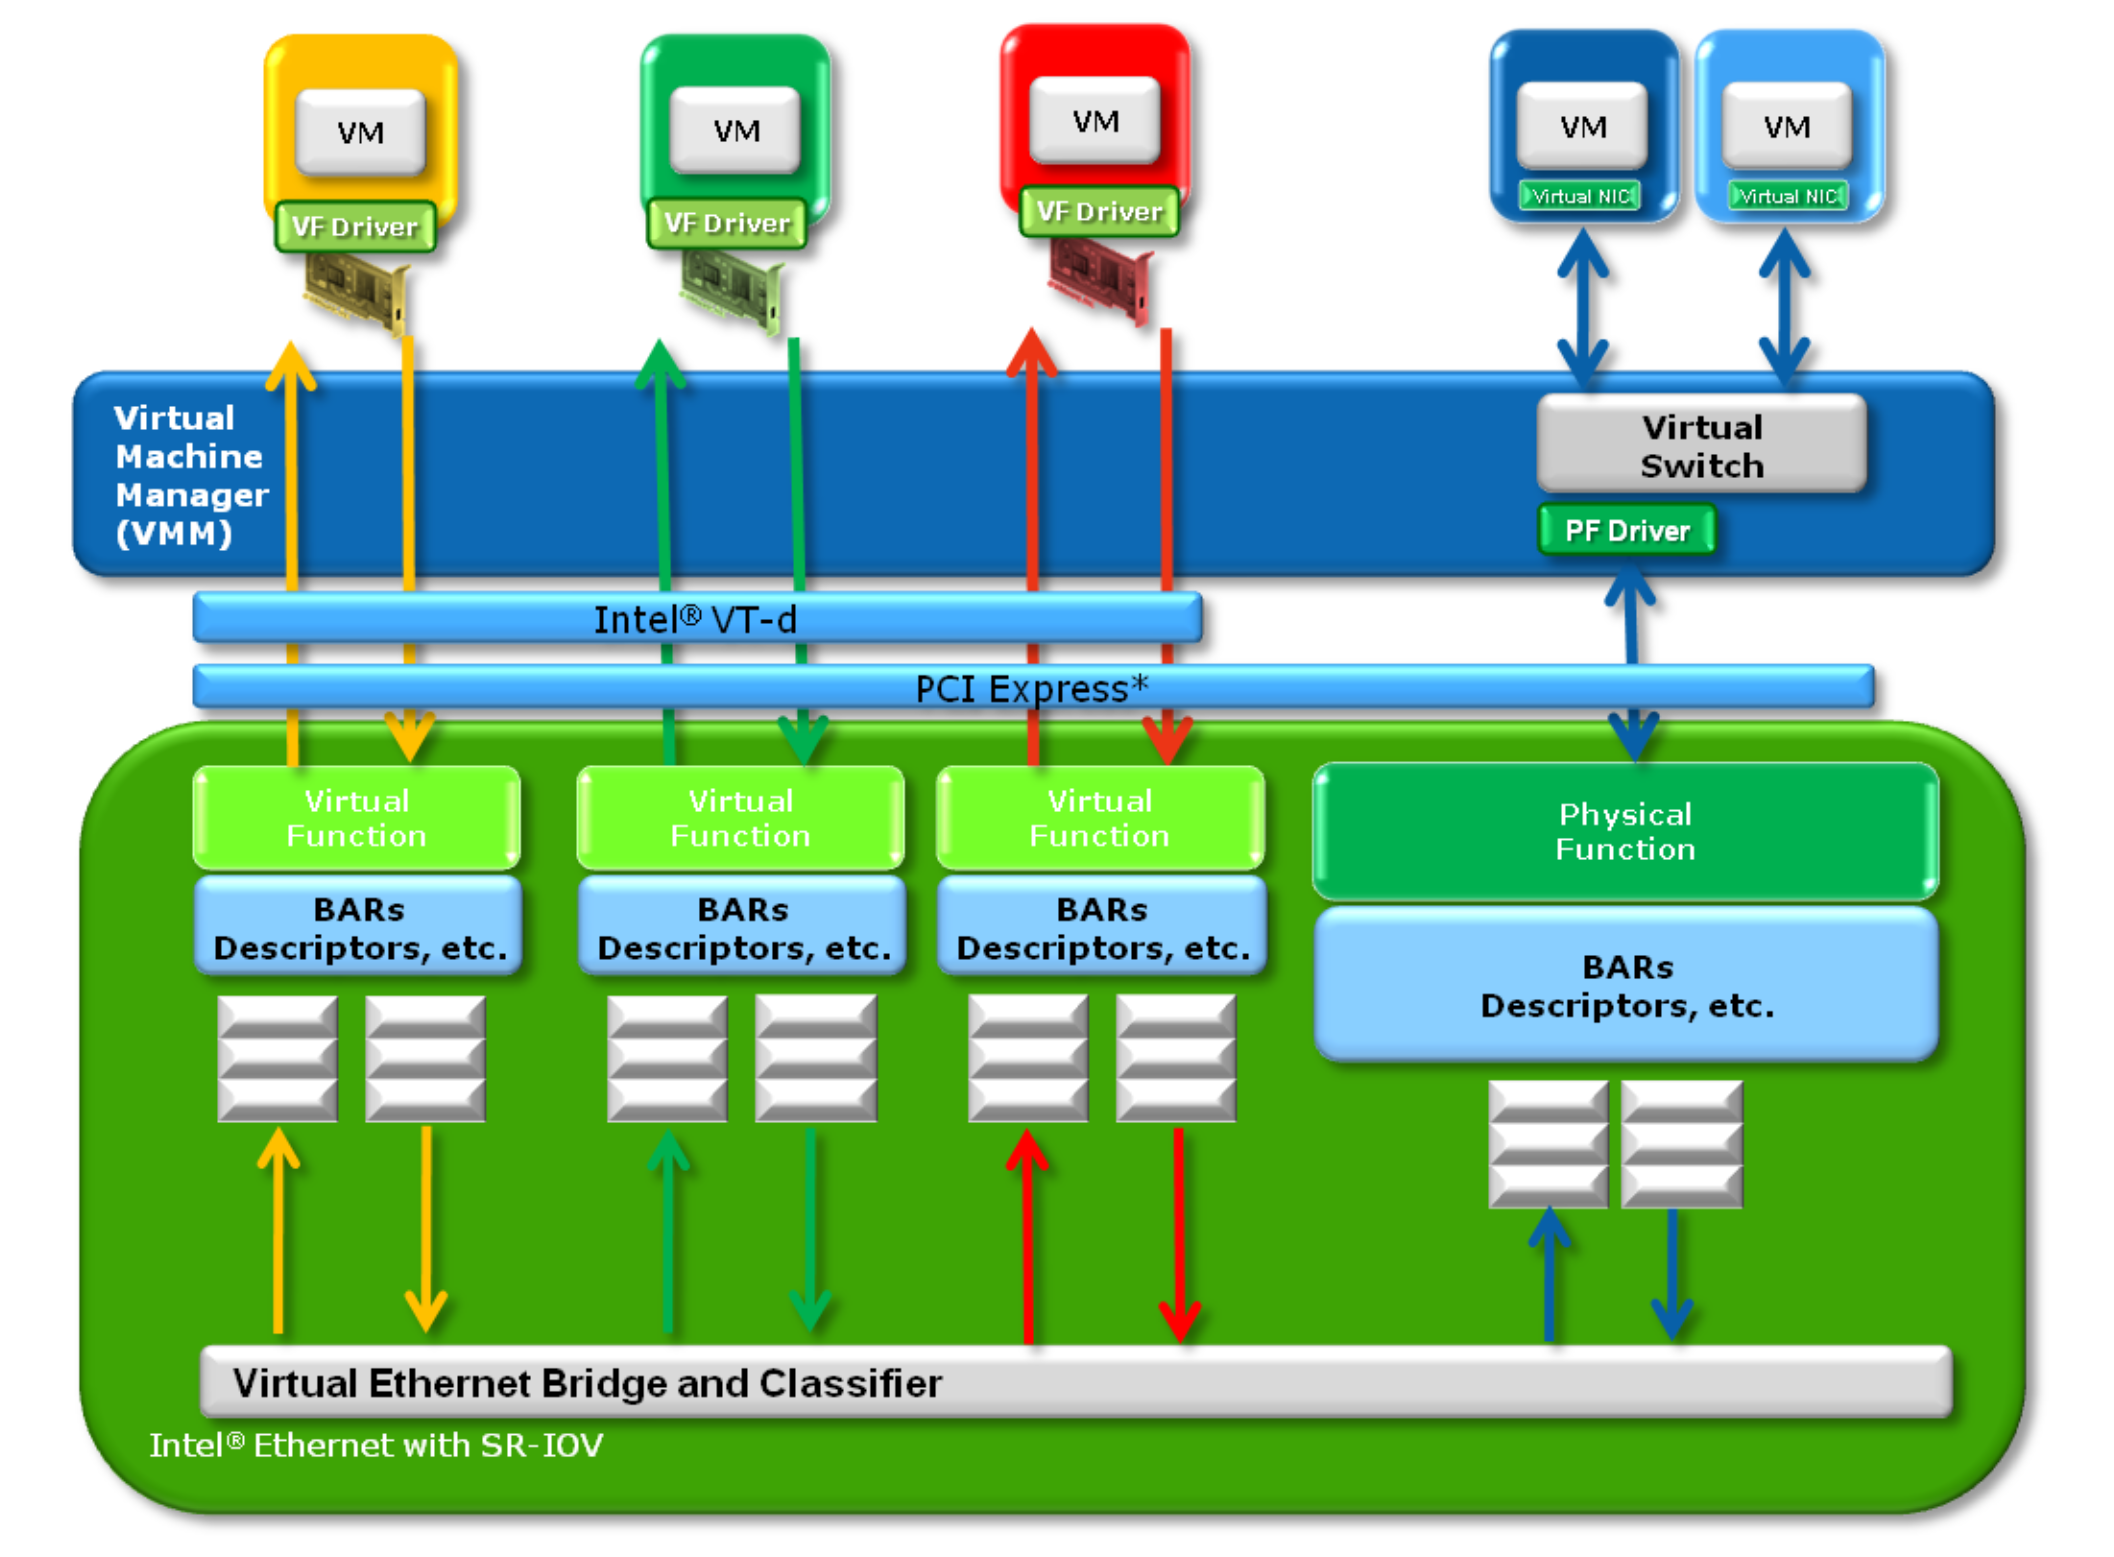
\includegraphics[width=1.0\textwidth]{resources/images/intel_sriov_Natively_and_Software_Shared.PNG}
	\caption{Natively (3 virtual machines on the left) and Software Shared \cite{intel_sriov}. The function type \textit{Virtual Function} (VF) can access a limited set of Base Address Register (BAR) descriptors (which holds the address of mapped memory of the device, or so called configuration space) and other parameters compared to the type \textit{Physical Function}. VF is designed to provide only the resources necessary for data movement.}
    \label{fig:related_work:intel_sriov_Natively_and_Software_Shared}
\end{figure}



\section{5G Data Plane enhancement with MTX}\index{5G Data Plane enhancement with MTX}
\label{sec:related_work:5g_dataplane_enhancement}
\Cref{fig:related_work:5g_dp_enhancement} describes how data is moved between \ac{UE} and \ac{DN} based on 3GPP specification and various sources.
A \ac{PDU} session is established to create a logical data path between \ac{UE} and \ac{UPF}.
This \ac{PDU} logical session runs on top of several transporting protocol.
Radio Bearer (RB) is the channel to move user data and control data between UE and radio equipment.
\ac{eCPRI} connects front-haul network and moves user data, controlling and management data, and synchronization data flows between DU and RU \cite{eCPRI_spec}.
\ac{gptu} connection - often called \textit{tunnel} - helps transferring user data between middle-haul and back-haul networks in UDP packets.
Data in different categories receive forwarding treatment differently, depends on the priority, subscription, ... 
This is managed by splitting the data into streams (called \ac{QoS} Flow, marked with QoS Flow Identification (QFI)), each is governed with different rule set (QoS rules).


\begin{figure}[H]
	\centering
	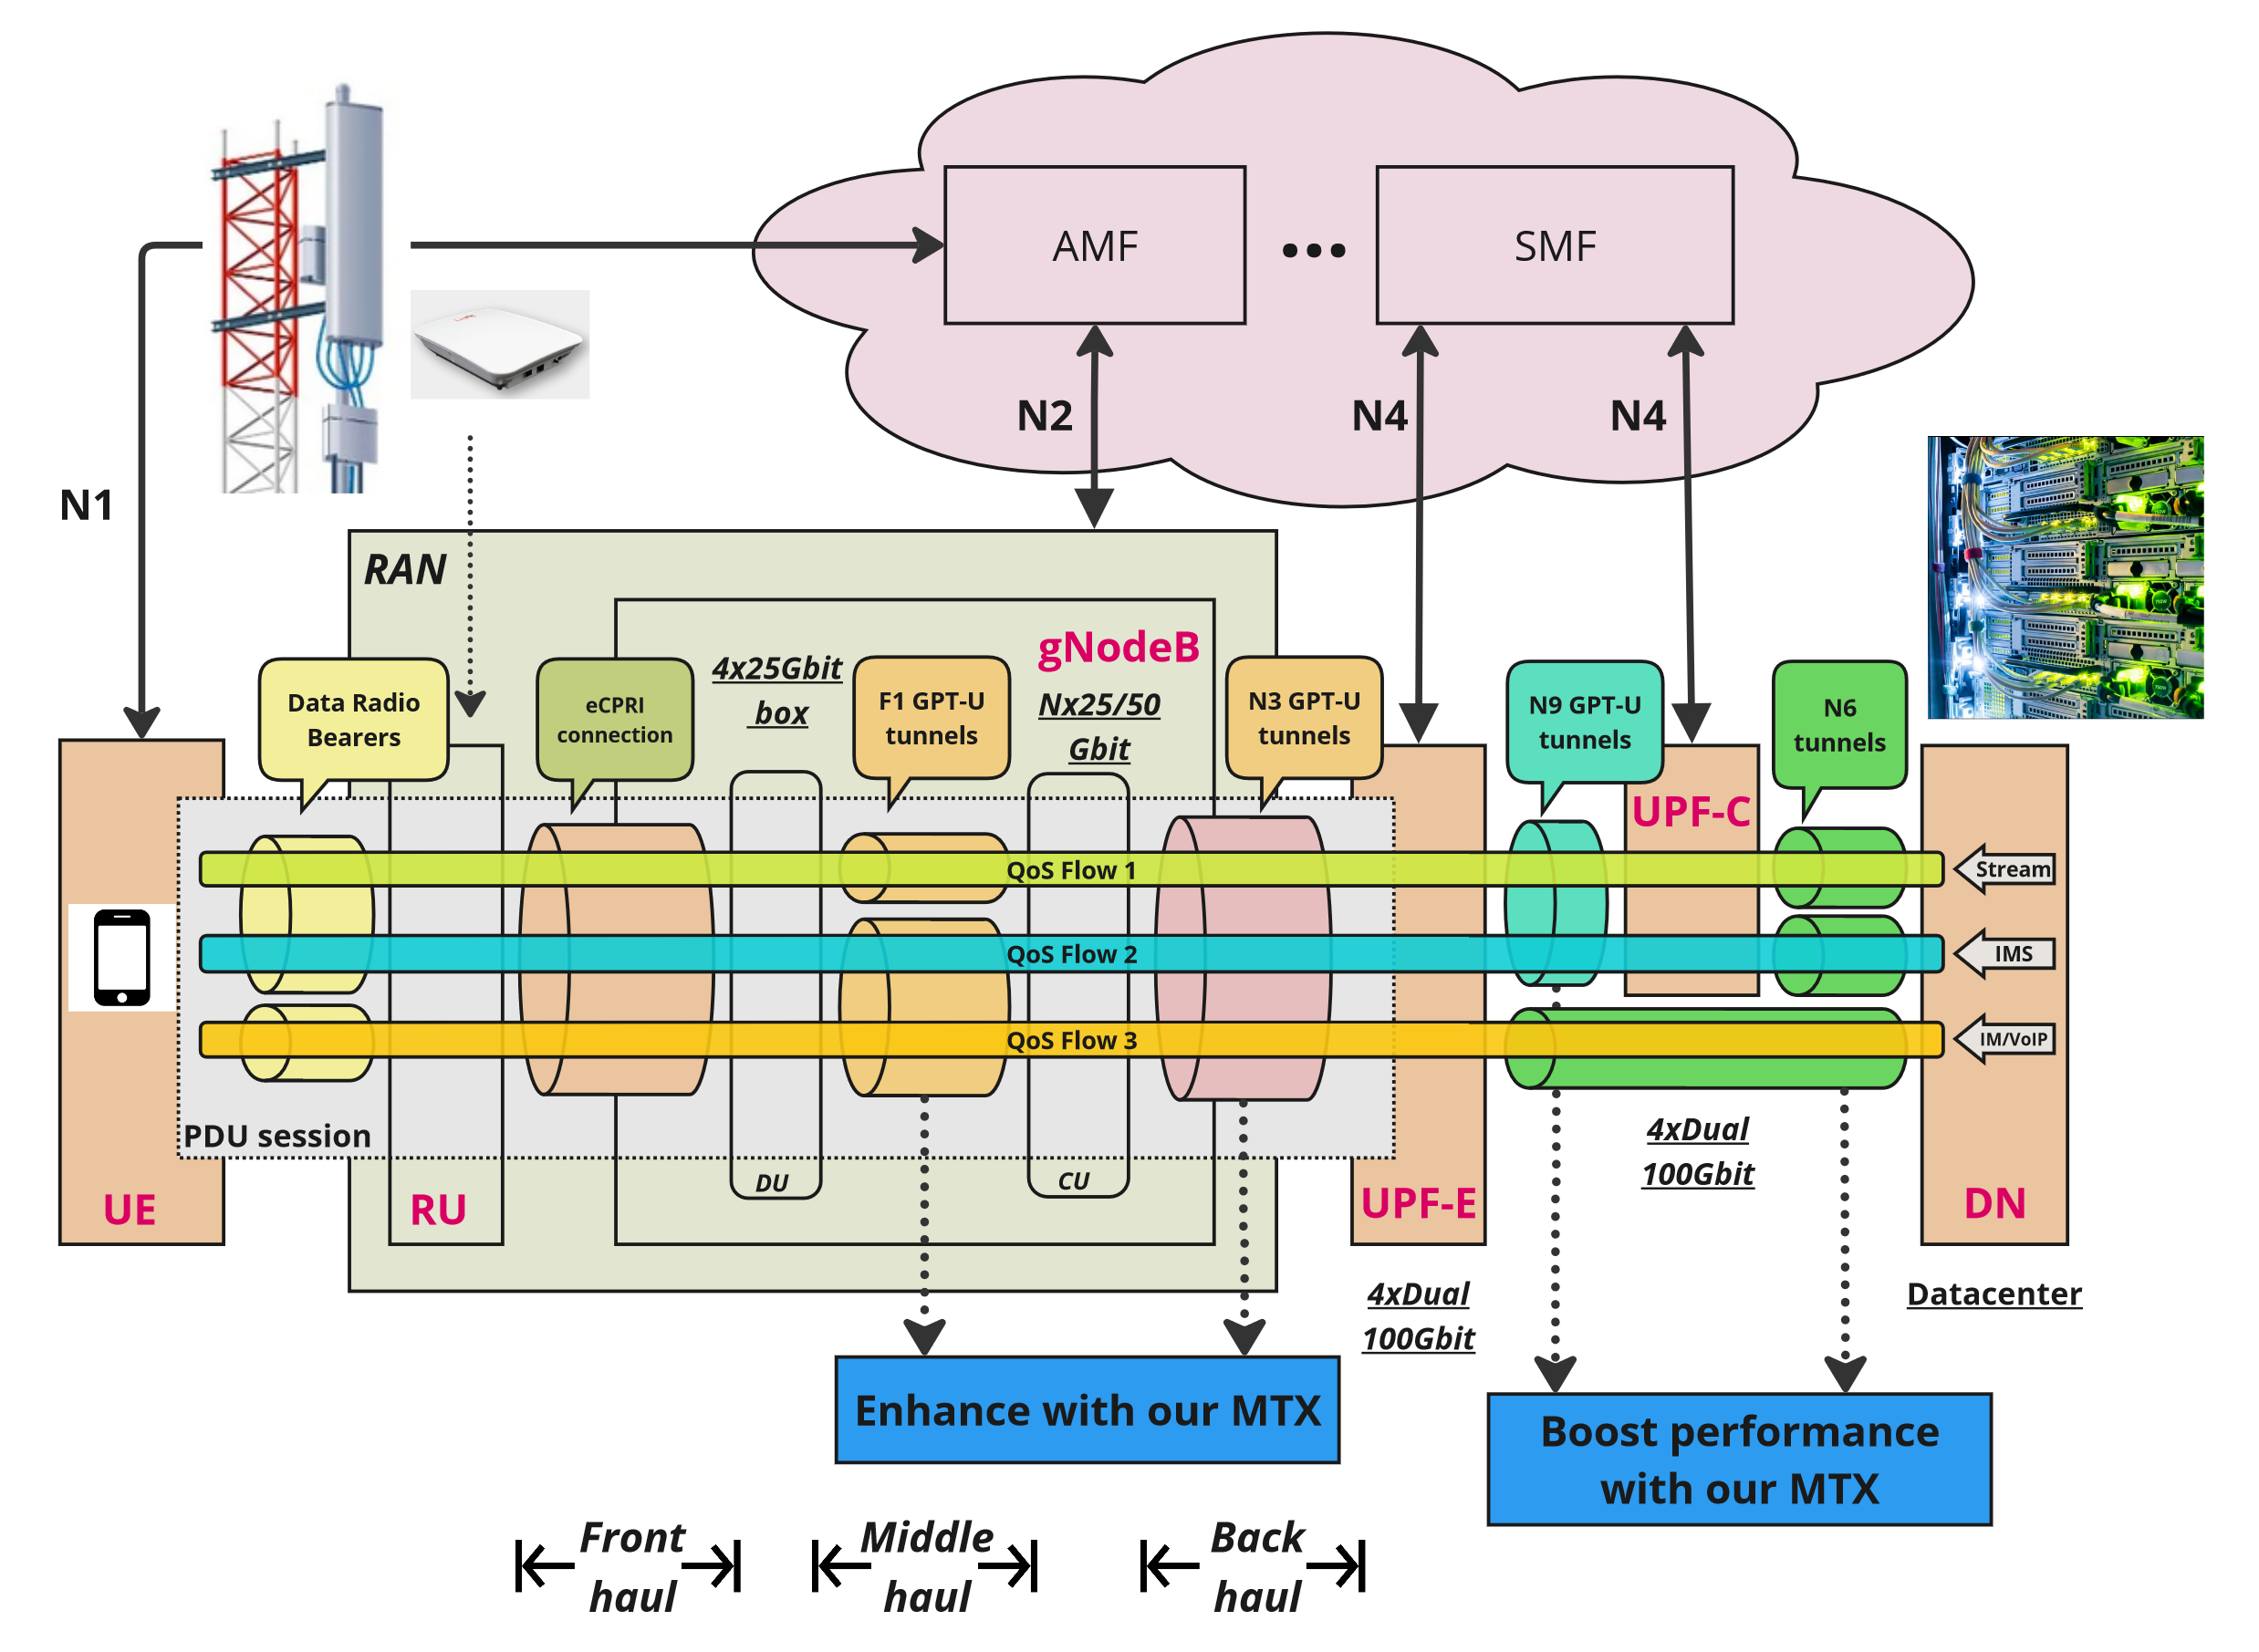
\includegraphics[width=1.0\textwidth]{resources/images/5g_dp_enhancement.PNG}
	\caption{5G Data Plane overview. The MTX library will be used as the building block for the GPT-U enhancement, which bring multipath capability to the protocol. Raw MTX can also be used to help connecting UPF and DN over multiple links.}
    \label{fig:related_work:5g_dp_enhancement}
\end{figure}

In actual deployed systems, \ac{gptu} tunnels are typically established and configured professionally on top of multiple links that are aggregated and managed by a software stack, for instance \ac{dpdkpage} and \ac{sriov}.
These solutions involve costly software and hardware (powerful and specifically chosen hardware) that lack flexibility, which make them unattractive for research and testing usage.
Open source implementations usually suffers from performance losses due to inefficiency, as noted in Open5GS discussion \cite{open5gs_github_dpdk}\cite{open5gs_github_udp_perf_cap}.

Our goal is to tackle the performance and usability issues by exploring the development of a straightforward yet robust multipath tunnel capable of functioning in both physical and virtual environments. 
To ensure ease of maintenance and facilitate compatibility with other protocols, we aim for a tunnel code base that remains simple and minimizes the need for extensive modifications, which is why \ac{xdppage} has been selected as the preferred transport method.
For the testing phase, we have chosen the \ac{gptu} protocol due to its diverse range of requirements that can be supported by MTX, including flow-awareness, high throughput, low latency, and a comprehensive set of configuration options.


\begin{figure}[H]
	\centering
	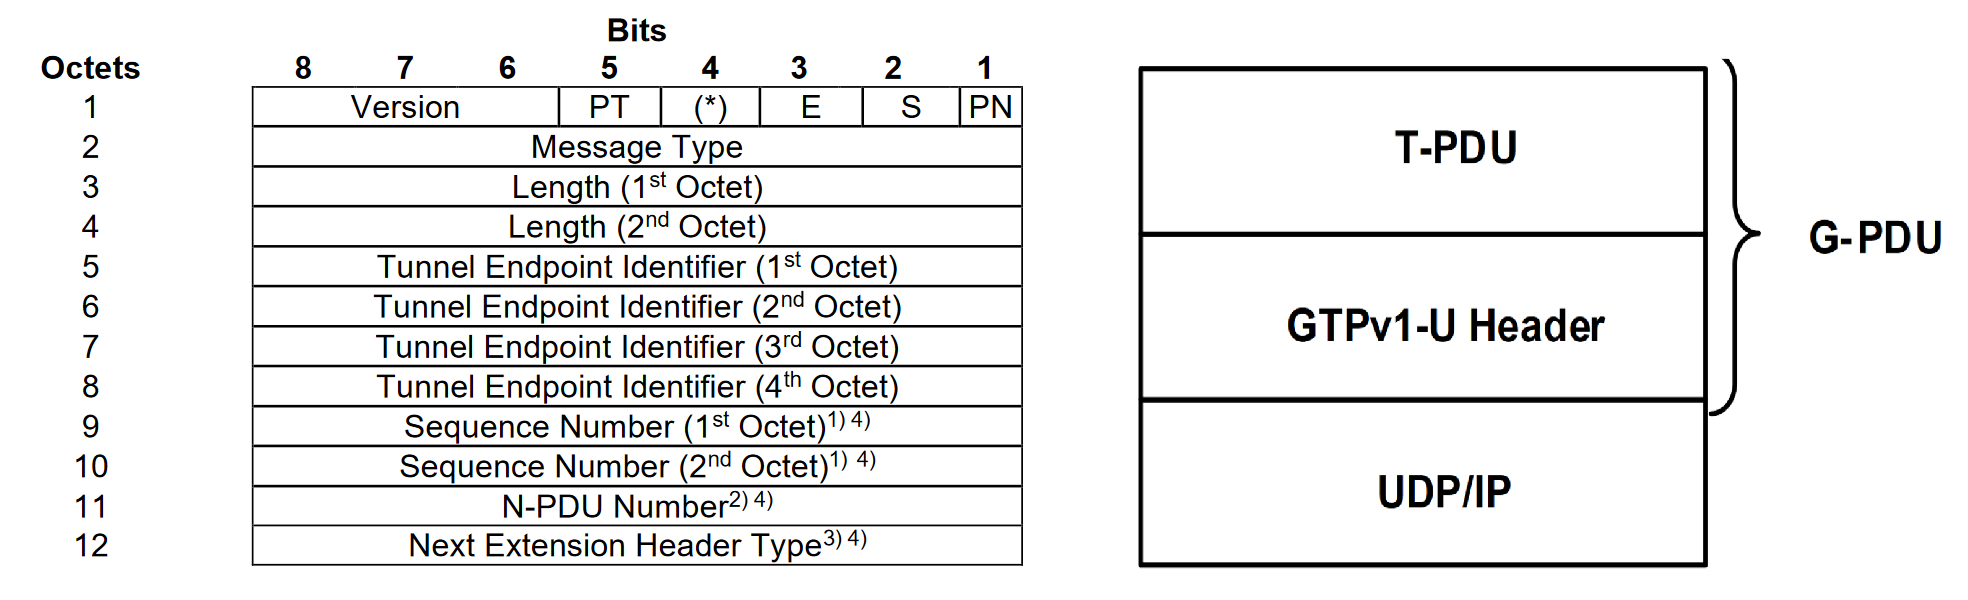
\includegraphics[width=1.0\textwidth]{resources/images/gptu_header_and_gpdu_stack.PNG}
	\caption{3GPP: GPT-U header and G-PDU Protocol Stack built on top of UDP/IP protocol \cite{3gpp_gptu}}
    \label{fig:related_work:gptu_header_and_gpdu_stack}
\end{figure}



% \begin{figure}[H]
% 	\centering
% 	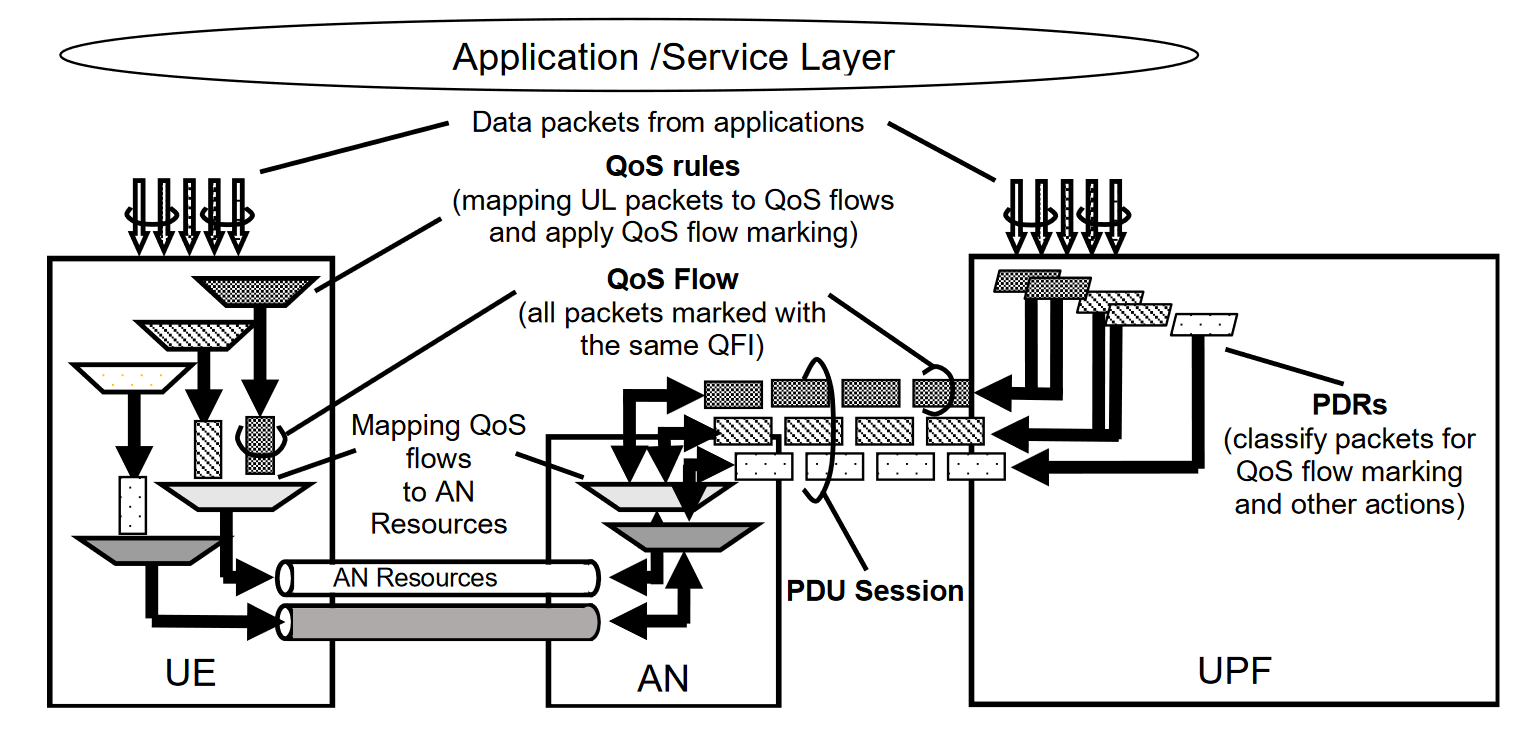
\includegraphics[width=1.0\textwidth]{resources/images/principle_for_classification_and__Plane_marking_for_QoS_Flows.PNG}
% 	\caption{The principle for classification and User Plane marking for QoS Flows and mapping
% 	to AN Resources \cite{3gpp_5g_system_architect_spec_release_18}}
%     \label{fig:related_work:principle_for_classification_and__Plane_marking_for_QoS_Flows}
% \end{figure}

% \begin{figure}[H]
%     \centering
%     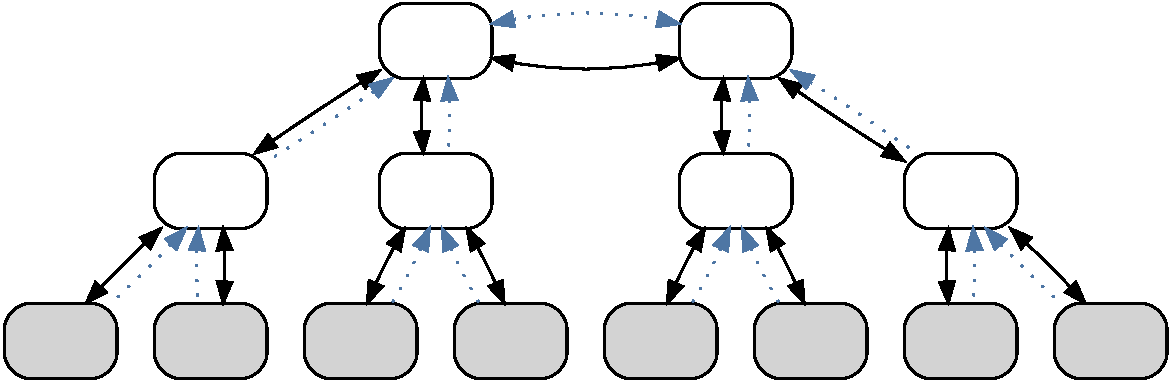
\includegraphics[width=.55\textwidth]{resources/images/example3}
%     \caption{Related area 1 within the structure of research}\label{fig:hourglass:ra1}
% \end{figure}

% \sidenote{Overview}
% \todomid{write about \Cref{fig:hourglass:ra1}}

% \sidenote{Focus}
% \todomid{write}

% \subsection{Specific Example 1}

% \sidenote{Definition}
% \todomid{write}

% \sidenote{Issues}
% \todomid{write}

% \subsection{Specific Example 2}

% \sidenote{Definition}
% \todomid{write}

% \sidenote{Implementations}
% \todomid{write}

% \sidenote{Research}
% \todomid{write}

% \sidenote{Standards}
% \todomid{write}

% \sidenote{Adoption}
% \todomid{write}

% \subsection{Specific Example 3}\index{Example 3}

% \sidenote{Transition}
% \todomid{write about \Cref{fig:sota:trans}}

% \begin{figure}
%     \centering
%     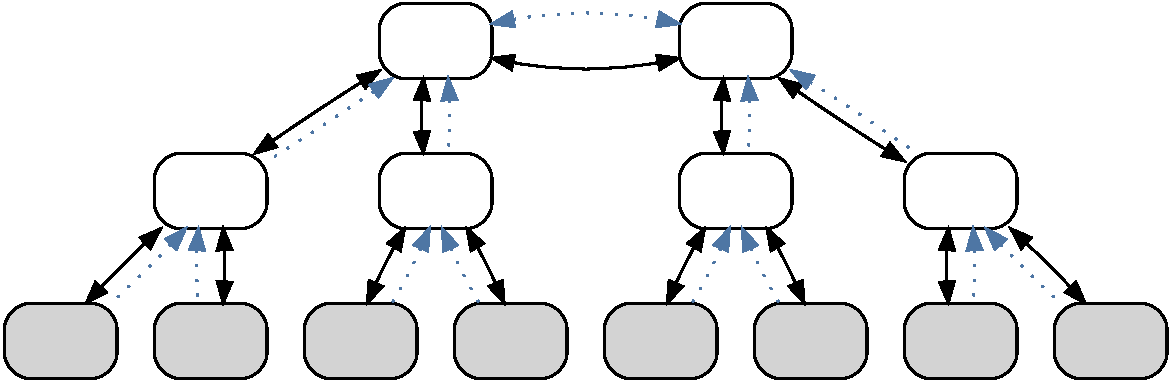
\includegraphics[width=.85\textwidth]{resources/images/example3}
%     \caption{Comparison of Example 2 and Example 3 (based on~\cite{li2002design})}\label{fig:sota:trans}
% \end{figure}

% \sidenote{Standards}
% \todomid{write}

% \sidenote{Extension}
% \todomid{write}

% \sidenote{Other Standards}
% \todomid{write}

% \sidenote{Something}
% \todomid{write}

% \sidenote{Something}
% \todomid{write}

% \sidenote{Something}
% \todomid{write}

% \sidenote{Something}
% \todomid{write}

% \sidenote{Something}
% \todomid{write}

% \sidenote{Something}
% \todomid{write}

% \section{Related Area 2}\index{Related Area 2}

% \sidenote{Overview}
% \todomid{write}

% \sidenote{Focus}
% \todomid{write about \Cref{fig:sota:ra2}}

% \begin{figure}[!hbtp]
%     \centering
%     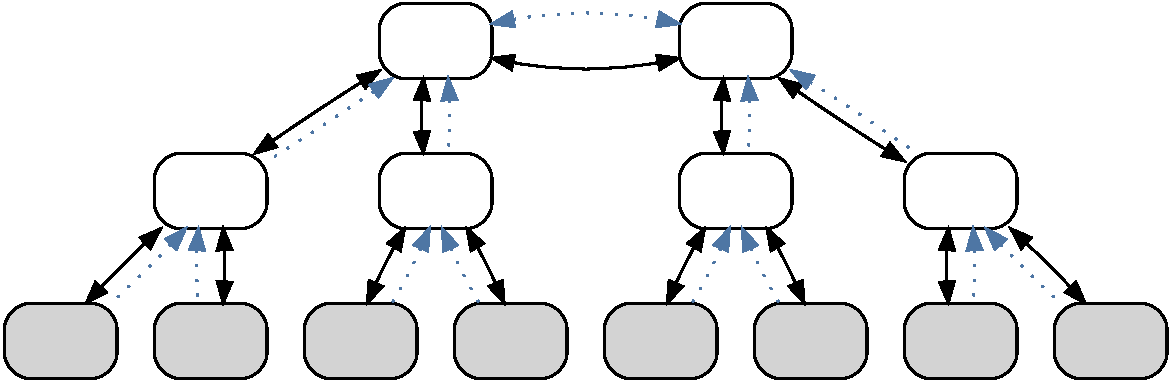
\includegraphics[width=1\textwidth]{resources/images/example3}
%     \caption{Related Area 2}\label{fig:sota:ra2}
% \end{figure}

% \sidenote{Something}
% \todomid{write}

% \subsection{Specific Example 1}

% \sidenote{Definition}
% \todomid{write}

% \sidenote{Issues}
% \todomid{write}

% \subsection{Specific Example 2}

% \sidenote{Definition}
% \todomid{write}

% \sidenote{Implementations}
% \todomid{write}

% \sidenote{Research}
% \todomid{write}

% \sidenote{Standards}
% \todomid{write}

% \sidenote{Adoption}
% \todomid{write}


% \section{Related Area 3}\index{Related Area 3}

% \sidenote{Overview}
% \todomid{write}

% \sidenote{Focus}
% \todomid{write about \Cref{fig:sota:ra3}}

% \begin{figure}[!hbtp]
%     \centering
%     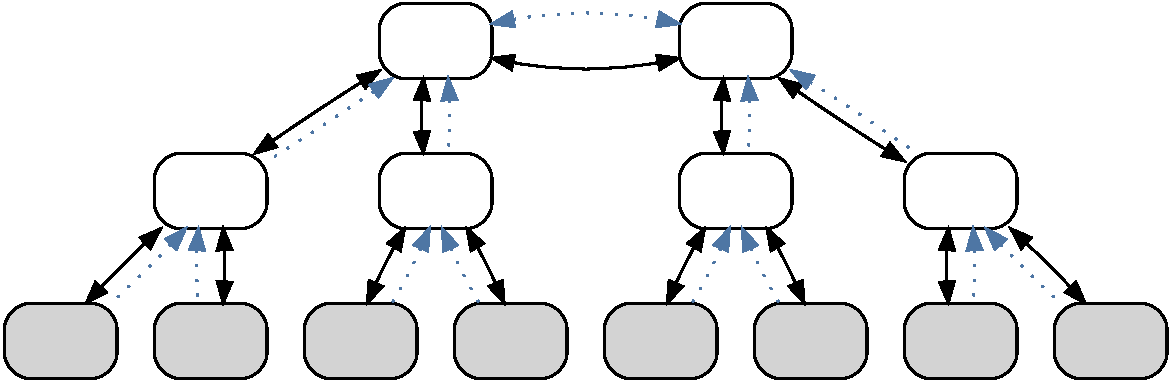
\includegraphics[width=1\textwidth]{resources/images/example3}
%     \caption{Related Area 3}\label{fig:sota:ra3}
% \end{figure}

% \sidenote{Something}
% \todomid{write}

% \subsection{Specific Example 1}

% \sidenote{Definition}
% \todomid{write}

% \sidenote{Issues}
% \todomid{write}

% \subsection{Specific Example 2}

% \sidenote{Definition}
% \todomid{write}

% \sidenote{Implementations}
% \todomid{write}

% \sidenote{Research}
% \todomid{write}

% \sidenote{Standards}
% \todomid{write}

% \sidenote{Adoption}
% \todomid{write}

% \section{Conclusion}

% \sidenote{Summary}
% \todomid{write}

% \sidenote{Takeaway 1}
% \todomid{write}

% \sidenote{Takeaway 2}
% \todomid{write}

% \sidenote{Takeaway 3}
% \todomid{write}

% \sidenote{Next chapter}
% \todomid{write}
